% This file was created with matplot2tikz v0.4.0.
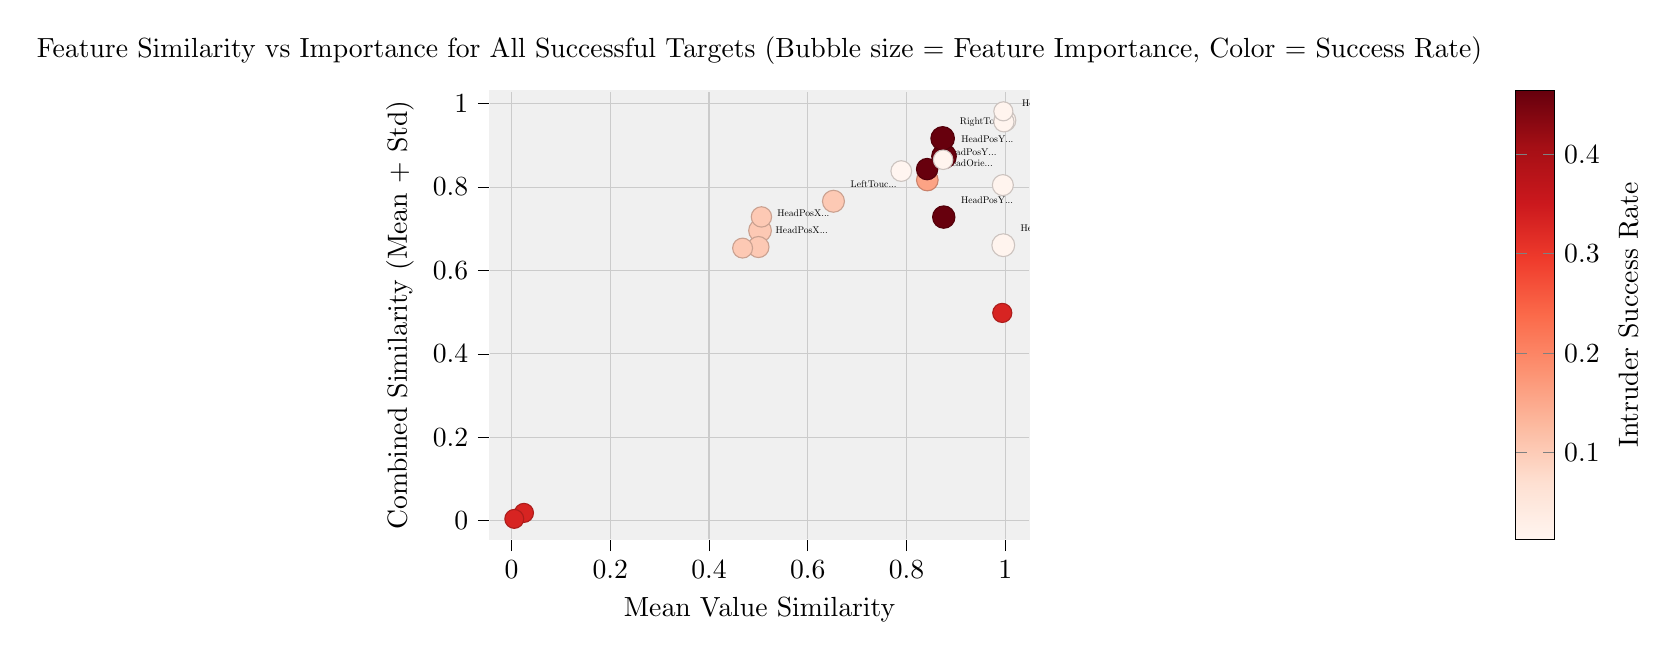
\begin{tikzpicture}

\definecolor{lightgray203}{RGB}{203,203,203}
\definecolor{whitesmoke240}{RGB}{240,240,240}

\begin{axis}[
axis background/.style={fill=whitesmoke240},
axis line style={whitesmoke240},
colorbar,
colorbar style={ylabel={Intruder Success Rate}},
colormap={mymap}{[1pt]
  rgb(0pt)=(1,0.96078431372549,0.941176470588235);
  rgb(1pt)=(0.996078431372549,0.87843137254902,0.823529411764706);
  rgb(2pt)=(0.988235294117647,0.733333333333333,0.631372549019608);
  rgb(3pt)=(0.988235294117647,0.572549019607843,0.447058823529412);
  rgb(4pt)=(0.984313725490196,0.415686274509804,0.290196078431373);
  rgb(5pt)=(0.937254901960784,0.231372549019608,0.172549019607843);
  rgb(6pt)=(0.796078431372549,0.0941176470588235,0.113725490196078);
  rgb(7pt)=(0.647058823529412,0.0588235294117647,0.0823529411764706);
  rgb(8pt)=(0.403921568627451,0,0.0509803921568627)
},
point meta max=0.463636363636364,
point meta min=0.0130434782608696,
tick align=outside,
tick pos=left,
title={Feature Similarity vs Importance for All Successful Targets
(Bubble size = Feature Importance, Color = Success Rate)},
x grid style={lightgray203},
xlabel={Mean Value Similarity},
xmajorgrids,
xmin=-0.0440117826165763, xmax=1.04900317958299,
xtick style={color=black},
y grid style={lightgray203},
ylabel={Combined Similarity (Mean + Std)},
ymajorgrids,
ymin=-0.044804011956461, ymax=1.03056702330372,
ytick style={color=black}
]
\addplot [
  colormap={mymap}{[1pt]
  rgb(0pt)=(1,0.96078431372549,0.941176470588235);
  rgb(1pt)=(0.996078431372549,0.87843137254902,0.823529411764706);
  rgb(2pt)=(0.988235294117647,0.733333333333333,0.631372549019608);
  rgb(3pt)=(0.988235294117647,0.572549019607843,0.447058823529412);
  rgb(4pt)=(0.984313725490196,0.415686274509804,0.290196078431373);
  rgb(5pt)=(0.937254901960784,0.231372549019608,0.172549019607843);
  rgb(6pt)=(0.796078431372549,0.0941176470588235,0.113725490196078);
  rgb(7pt)=(0.647058823529412,0.0588235294117647,0.0823529411764706);
  rgb(8pt)=(0.403921568627451,0,0.0509803921568627)
},
  only marks,
  scatter,
  scatter src=explicit,
  scatter/@pre marker code/.append style={/tikz/mark size=\perpointmarksize},
  visualization depends on={\thisrow{sizedata} \as\perpointmarksize}
]
table [x=x, y=y, meta=colordata]{%
x  y  colordata  sizedata
0.876068699972893 0.873842249113757 0.4636363636363636 4.4509969756607335
0.873289871579181 0.916727988721059 0.4636363636363636 4.258414740696401
0.996063475134934 0.660565925510998 0.016 4.126520855754281
0.50339951193751 0.695665230964297 0.104 4.108745096166149
0.875548448002787 0.728002223854182 0.4636363636363636 4.041039106279105
0.652122806592537 0.765973794252133 0.104 3.9706039345831523
0.999320681301193 0.959944287929977 0.016 3.964958667415685
0.842261262773048 0.816887080994658 0.1590909090909091 3.9066565469201664
0.841856823907129 0.843090704279384 0.4636363636363636 3.858494440449224
0.500245985876548 0.656171642725335 0.104 3.8083628905933073
0.99523310500907 0.804701098384301 0.016 3.797042709514804
0.7894920809477 0.83843320628509 0.013043478260869565 3.74178192080743
0.506290164754489 0.728403454081083 0.104 3.6784535998994827
0.997410005054446 0.956557811461731 0.016 3.653063123057029
0.468106606528771 0.65364066806129 0.104 3.602693640355186
0.874252330005344 0.865547114354053 0.016 3.523381873335605
0.994053667370903 0.498173718667341 0.33181818181818185 3.458903718487564
0.996223646237148 0.981686521700983 0.016 3.4511706220048866
0.0252525688264241 0.0184517398230062 0.33181818181818185 3.4442126710430463
0.00567071566522226 0.00407648964627444 0.33181818181818185 3.4199830307239556
};
\draw (axis cs:0.876068699972893,0.873842249113757) ++(5pt,5pt) node[
  scale=0.35,
  anchor=base west,
  text=black,
  rotate=0.0
]{HeadPosY...};
\draw (axis cs:0.873289871579181,0.916727988721059) ++(5pt,5pt) node[
  scale=0.35,
  anchor=base west,
  text=black,
  rotate=0.0
]{RightTou...};
\draw (axis cs:0.996063475134934,0.660565925510998) ++(5pt,5pt) node[
  scale=0.35,
  anchor=base west,
  text=black,
  rotate=0.0
]{HeadPosY...};
\draw (axis cs:0.50339951193751,0.695665230964297) ++(5pt,5pt) node[
  scale=0.35,
  anchor=base west,
  text=black,
  rotate=0.0
]{HeadPosX...};
\draw (axis cs:0.875548448002787,0.728002223854182) ++(5pt,5pt) node[
  scale=0.35,
  anchor=base west,
  text=black,
  rotate=0.0
]{HeadPosY...};
\draw (axis cs:0.652122806592537,0.765973794252133) ++(5pt,5pt) node[
  scale=0.35,
  anchor=base west,
  text=black,
  rotate=0.0
]{LeftTouc...};
\draw (axis cs:0.999320681301193,0.959944287929977) ++(5pt,5pt) node[
  scale=0.35,
  anchor=base west,
  text=black,
  rotate=0.0
]{HeadPosY...};
\draw (axis cs:0.842261262773048,0.816887080994658) ++(5pt,5pt) node[
  scale=0.35,
  anchor=base west,
  text=black,
  rotate=0.0
]{HeadOrie...};
\draw (axis cs:0.841856823907129,0.843090704279384) ++(5pt,5pt) node[
  scale=0.35,
  anchor=base west,
  text=black,
  rotate=0.0
]{HeadPosY...};
\draw (axis cs:0.500245985876548,0.656171642725335) ++(5pt,5pt) node[
  scale=0.35,
  anchor=base west,
  text=black,
  rotate=0.0
]{HeadPosX...};
\end{axis}

\end{tikzpicture}
